\section{Stimulated qubit transitions}

The visibility of the qubit state measurement increases as we collect more scattered photons.
Therefore, probing the measurement circuit with a higher power pulse should lead to better measurement visibility.
However, at large numbers the resonator photons induce qubit transitions between the $\ket{0}$ and $\ket{1}$ states \cite{Johnson:heralding2012, Slichter:dressedDephasing2012}.
To determine how hard we could drive the measurement system without disrupting the qubit, we measured the qubit state transitions as a function of resonator drive power .
We prepared the qubit in either $\ket{0}$ or $\ket{1}$ and then applied a measurement pulse with variable power.
We then allowed the resonator to ring down, and finally probed the resonator with a measurement pulse to determine the state of the qubit.
The pulse sequence is illustrated in Fig.\,\ref{Fig:ch:results:sec:stimulatedTransitions:stimulatedTransitions_1D}\,a.
In this way we measured the probability of a qubit transition from initial states $\left\{ \ket{0}, \ket{1} \right\}$ to final states $\left\{ \ket{0}, \ket{1}, \ket{2} \right\}$ as a function of the driving DAC amplitude.
We then converted the DAC amplitude to resonator photon number using the ac Stark shift calibration. 

We observe a sharp onset of stimulated qubit state transitions at sufficiently high photon numbers, as shown in Fig.\,\ref{Fig:ch:results:sec:stimulatedTransitions:stimulatedTransitions_1D}\,b.
As shown in Fig\,\ref{Fig:ch:results:sec:stimulatedTransitions:stimulatedTransitions_1D}\,b, $\ket{1}\rightarrow\ket{0}$ transitions set in abruptly at $n \gtrsim 100$.
The complementary transition, $\ket{0}\rightarrow\ket{1}$ sets in at $n \gtrsim 175$.
Note also that we observed transitions to $\ket{2}$ from both initial states.

At low photon numbers, the probabilities for no transition, such as $\ket{0}\rightarrow\ket{0}$, are not 1.
The main contributing factor to this is that when idle, the qubits are not perfectly in the ground state.
We observe between 4\% and 8\% idle $\ket{1}$ population, which means that the $\ket{0}\rightarrow\ket{0}$ probability will be no greater than 0.92-0.96.
This same effect raises the $\ket{1}\rightarrow\ket{0}$ at low photon numbers: if the qubit is erroneously prepared in $\ket{1}$, then a $\pi$-pulse intended to prepare $\ket{1}$ instead puts the qubit in $\ket{0}$.
This process manifests as a nonzero probability for $\ket{1}\rightarrow\ket{0}$ at low photon number.

We used these data to choose the maximum usable photon number.
As a rule of thumb, we kept the photon number at $1/2$ the value of the sharp onset of qubit state transitions.
The exact value depended on the values of $g$ for each qubit, and the operating value of $\Delta$.
Later, in our analysis of the time dependent measurement fidelity, we will see that the fidelity numbers themselves place a strong bound on the probability of stimulated qubit transitions, providing further indication that our experiments were done at values of $n$ which preserved the qubit state.

\begin{figure}
\begin{centering}
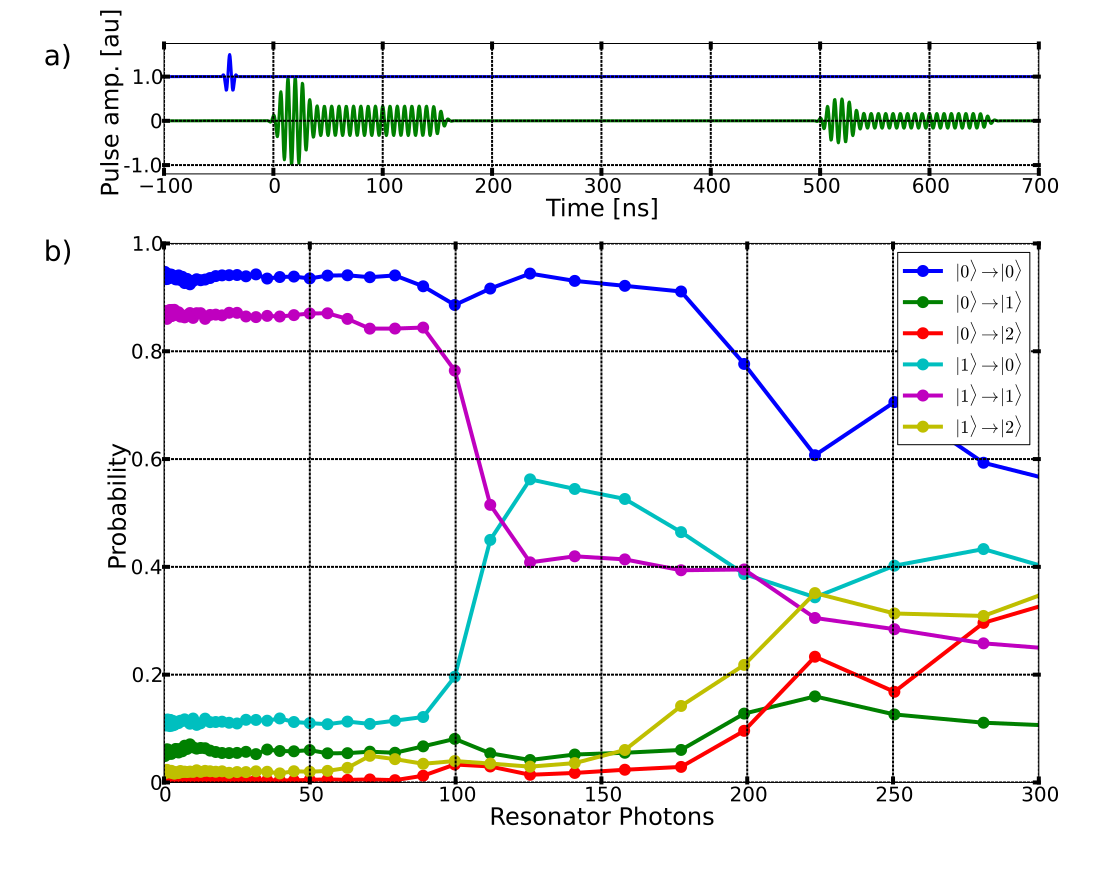
\includegraphics[width=\textwidth]{stimulatedTransitions_1D.pdf}
\par\end{centering}
\caption{Qubit transitions stimulated by the measurement pulse. a) Pulse sequence. The qubit is prepared into the $\ket{0}$ ($\ket{1}$) state with an idle ($\pi$-pulse) as shown in blue. We then drive the measurement resonator with a variable power pulse, as shown in green. This pulse can induce qubit state transitions. After a ring-down period, we probe the measurement resonator with a low power pulse to measure the state of the qubit. b) Probabilities for the final state of the qubit for initial states $\ket{0}$ or $\ket{1}$. Each curve labelled $\ket{i}\rightarrow\ket{f}$ gives the probability that the qubit prepared in state $\ket{i}$ is measured at the end of the sequence to be in state $\ket{f}$.}
\label{Fig:ch:results:sec:stimulatedTransitions:stimulatedTransitions_1D}
\end{figure}


\subsection{Comparison with theory}

In the dispersive Hamiltonian given in Eq.\,(\ref{eq:dispersiveHamiltonianInteraction}), the photon number operator $n$ couples only to the qubit $\sigma_z$.
Therefore, resonator photons should not induce upward or downward transitions of the qubit state.
Our treatment of the dispersive limit assumes $g / \Delta \ll 1$, but ignores the additional dimensionless factor of $n$ itself.
This suggests that at large values of $n$, our lowest order expansion becomes insufficient and other terms involving qubit transitions via $\sigma_x$ or $\sigma_y$ may appear.
We do not give a full account of this physics, but comment on how the critical $n$ found in our data relates to rough theoretical predictions.
The dispersive Hamiltonian is an expansion to first order in $(g/\Delta)^2$.
Therefore, we might expect qubit transitions for $n > (\Delta / g)^2$.
In the literature, the critical photon number is defined as $n_{\text{crit}} \equiv (\Delta/g)^2 / 4$.
In the present experiment we have $n_{\text{crit}} \approx 30$.
Interestingly, we do not observe stimulated transitions until $n \approx 3 \, n_{\text{crit}}$.


%\subsection{Time dependence}
%
%We have also made preliminary measurements of the time dependence of the stimulated transitions by varying the length of the stimulation pulse.
%We found a slight dependence of the stimulated transitions on the pulse length, as shown in Fig.\,\ref{Fig:ch:results:sec:stimulatedTransitions:stimulatedTransitions_2D}.
%Unfortunately, the photon number calibration for these data was found during the analysis phase to be unreliable.
%However, one very interesting feature can still be extracted.
%With increasing pulse length, we find increased 
%
%\begin{figure}
%\begin{centering}
%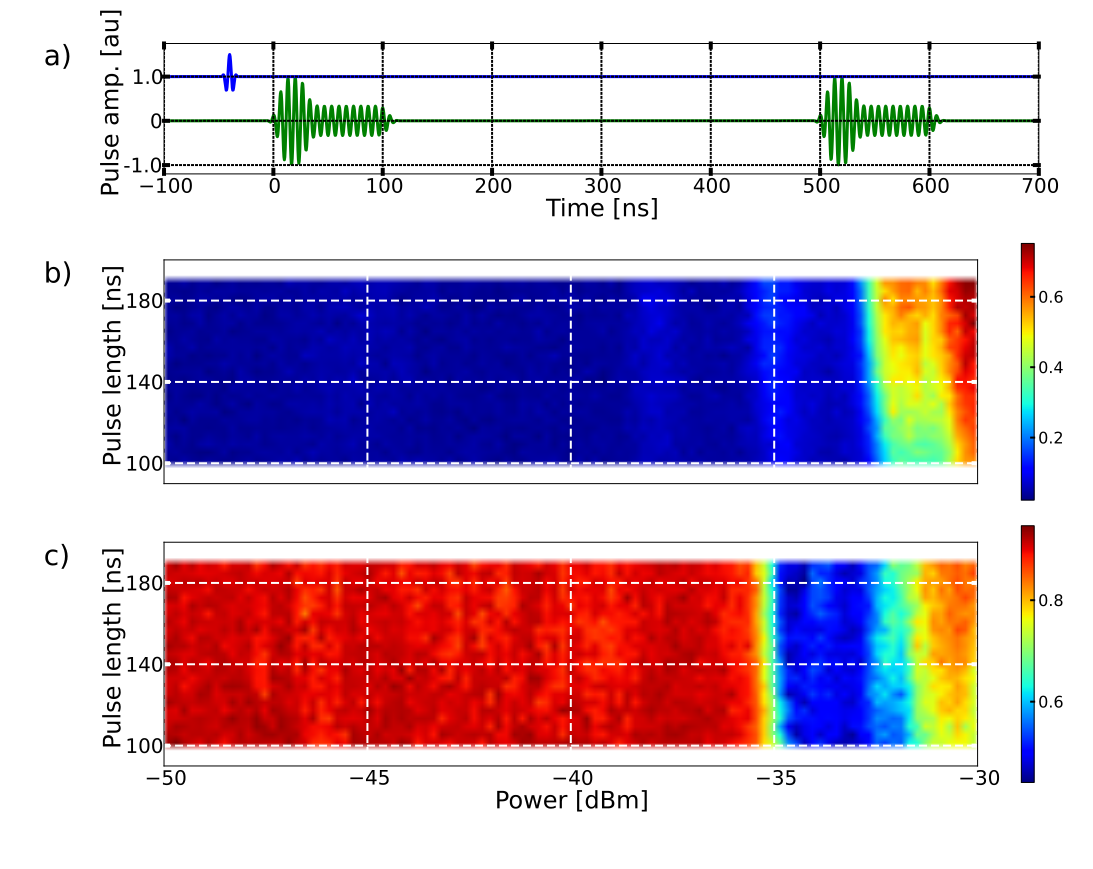
\includegraphics[width=\textwidth]{stimulatedTransitions_2D.pdf}
%\par\end{centering}
%\caption{...}
%\label{Fig:ch:results:sec:stimulatedTransitions:stimulatedTransitions_2D}
%\end{figure}

To our knowledge, neither the precise photon number at which qubit transitions are induced, nor even the sharp onset with increasing $n$ has been understood in the theoretical literature.
Characterization and theoretical understanding of this effect would be a natural continuation of the present work.
